\documentclass{beamer}
\usetheme{Madrid}
\usecolortheme{beaver}
\usepackage[francais]{babel}
\usepackage[utf8]{inputenc} % Required for including letters with accents
\usepackage[T1]{fontenc} % Use 8-bit encoding that has 256 glyphs
\usepackage{pythontex}
\usepackage{amsthm}
\usepackage{amsmath}
\usepackage{amssymb}
\usepackage{mathrsfs}
\usepackage{graphicx}
\usepackage{geometry}
\usepackage{stmaryrd}
\usepackage{tikz}
\usetikzlibrary{patterns}
%\usetikzlibrary{intersections}

\usepackage{stmaryrd}
%\usepackage{tikz}
%\usetikzlibrary{tikzmark}
\usepackage{empheq}
\usepackage{longtable}
\usepackage{booktabs} 
\usepackage{array}
\usepackage{pstricks}
\usepackage{pst-3dplot}
\usepackage{pst-tree}
\usepackage{pstricks-add}
\usepackage{upgreek}
%\usepackage{epstopdf}
\usepackage{eolgrab}
\usepackage{chngpage}
 \usepackage{calrsfs}
 % Appel du package pythontex 
\usepackage{pythontex}





\usetikzlibrary{decorations.pathmorphing}
\def \de {{\rm d}}
\usepackage{color}
\usepackage{xcolor}
\newcommand{\mybox}[1]{\fbox{$\displaystyle#1$}}
\newcommand{\myredbox}[1]{\fcolorbox{red}{white}{$\displaystyle#1$}}
\newcommand{\mydoublebox}[1]{\fbox{\fbox{$\displaystyle#1$}}}
\newcommand{\myreddoublebox}[1]{\fcolorbox{red}{white}{\fcolorbox{red}{white}{$\displaystyle#1$}}}
%\usetheme[options]{Boadilla}

  \title{Introduction aux éléments finis}
  \author{ \textsc{Ibrahim ALAME}}\institute{ESTP}
\date{24/09/2021}
  \begin{document}
 \begin{frame}
  \titlepage
  \end{frame}
  
\begin{frame}
\frametitle{Bref historique de la méthode}

\begin{itemize}
\item issue des travaux de Courant ($\sim$1930)
\item développée par les ingénieurs en aéronautique ($\sim$1950)
\item analysée dans les années $\sim$1970
\item utilisée dans de multiples applications (cf. cours de Mécanique)
Richard Courant (1888-1972)
\begin{center}
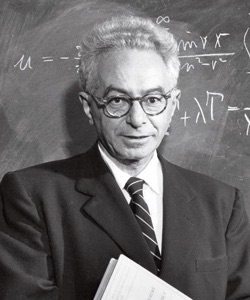
\includegraphics[scale=0.3]{courant.jpg} 
\end{center}
\end{itemize}
\end{frame}
%%%%%%%%%%%%%%%%%%%%%%%%%%%%%%%%%%%%%%%%%%%%%%%%%%%%%%%
\begin{frame}
\frametitle{Outils d'analyse fonctionnelle }
\begin{itemize}
\item \underline{Rappels sur les distributions}
\item \underline{Espaces de Sobolev}
\[\displaystyle H^1(\Omega)=\{v\in L^2(\Omega), \frac{\partial v}{\partial x_i} \in L^2(\Omega)\}\]
\[H_0^1(\Omega)=\{v\in H^1(\Omega), v_{/\Gamma}=0\}\]
muni de la norme
\[\|v\|_{H^1}^2=\left(\int_{\Omega}v^2 + \int_{\Omega} |\nabla v|^2\right)=(\|v\|_{L^2}^2+\|\nabla v\|_{L^2}^2)\]
$H^1(\Omega)$ est un espace de Hilbert.

 Plus généralement $H^m(\Omega)=\{v\in L^2(\Omega), \partial^\alpha v\in L^2(\Omega), |\alpha|\leq m\}$.
\item \underline{Formule de Green:}
\[-\int_\Omega \Delta u\cdot v \; \de x = \int_\Omega \nabla u\cdot \nabla v \; \de x-\int_\Gamma  \frac{\partial u}{\partial \vec n} \cdot v \; \de \sigma\]
\end{itemize}

\end{frame}


\begin{frame}
\frametitle{Problème modèle}
\begin{itemize}
\item Membrane élastique à l'équilibre sous un chargement
\begin{center}
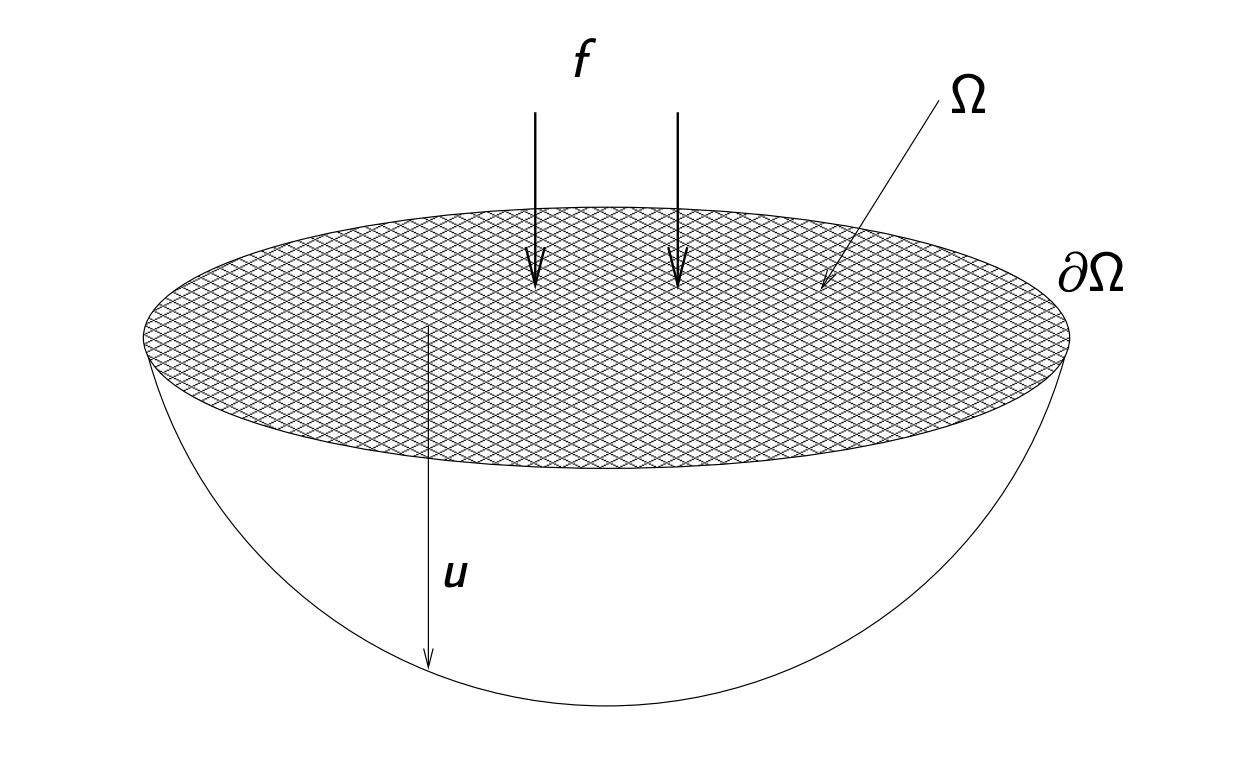
\includegraphics[scale=0.2]{membrane00.png} 
\end{center}
\begin{itemize}
\item membrane tendue occupant le domaine $\Omega\subset\mathbb{R}^2$
\item fixée sur son pourtour
\item on applique un chargement vertical $f$
\end{itemize}
\item L'inconnue est le déplacement vertical de la membrane à l'équilibre
\[u:\Omega \to \mathbb{R}\]
\item La fonction $u$ est solution du problème aux limites
\begin{equation}
\left\{
\begin{array}{l}
-\Delta u = f \mbox{ dans } \Omega \quad \mbox{ bilan des forces }\\
u=0  \mbox{ sur } \partial \Omega \quad \mbox{ condition limite }
\end{array}
\right.
\label{dirichletDim1}
\end{equation}
\end{itemize}

\end{frame}



\begin{frame}
\frametitle{Formulation variationnelle}
\begin{itemize}
\item $-\Delta u = f  \Longrightarrow -\Delta u \cdot v= f \cdot v \quad \mbox{ où }v\in H_0^1(\Omega)$
\[\displaystyle -\int_{\Omega}\Delta u \cdot v \; \de x= \int_{\Omega}f \cdot v \; \de x\]
\[ \int_\Omega \nabla u\cdot \nabla v \; \de x-\int_\Gamma  \frac{\partial u}{\partial \vec n} \cdot v \; \de \sigma = \int_{\Omega}f \cdot v \; \de x\]
\[ \int_\Omega \nabla u\cdot \nabla v \; \de x = \int_{\Omega}f \cdot v \; \de x\]
\item Formulation variationnelle (cf. cours d'analyse)
\begin{equation}
\myredbox{
\left\{
\begin{array}{l}
\mbox{Trouver } u \in H_0^1(\Omega)\;\mbox{ tel que }\\
\displaystyle \int_{\Omega}\nabla u\cdot \nabla v = \int_{\Omega}f v \quad \forall v\in H_0^1(\Omega) 
\end{array}
\right.}
\label{formVar1}
\end{equation}
\begin{itemize}
\item principe des travaux virtuels
\item $v$ est la fonction test
\end{itemize}

\end{itemize}


\end{frame}





%%%%%%%%%%%%%%%%%%%%%%%%%%%%%%%%%%%%%%%%%%
\begin{frame}
\frametitle{Théorème de Lax-Milgram}
\begin{itemize}
\item Le problème abstrait
\begin{equation}
\left\{
\begin{array}{l}
\mbox{Trouver } u \in V\;\mbox{ tel que }\\
a(u,v)= \ell(v) \quad \forall v\in V
\end{array}
\right.
\label{probAbst1}
\end{equation}
est bien posé sous les conditions (suffisantes) suivantes :
\begin{description}
\item[LM1]  l'espace V équipé de la norme $\|\cdot\|_V$ est un espace de Hilbert
\item[LM2]  la forme linéaire $\ell$ est continue sur $V$
\[\exists\beta,\quad \forall v \in V,\quad |\ell(v)\leq \beta \|v\|_V\]
\item[LM3]  la forme bilinéaire $a(\cdot,\cdot)$ est continue sur $V \times V$
\[\exists \omega,\quad \forall v,\, w\in V,\quad |a(v,w)\leq \omega\; \|v\|_V \cdot \|w\|_V\]
\item[LM4] la forme bilinéaire a est coercive sur $V$
\[\exists\alpha,\quad \forall v \in V,\quad a(v,v)\geq \beta \|v\|^2_V\]
\end{description}

\end{itemize}
\end{frame}

\begin{frame}
\frametitle{Application à l'équilibre d'une membrane}
\begin{itemize}
\item On suppose $f\in L^2(\Omega)$
\item Le problème \eqref{formVar1} est bien posé. En effet,
\end{itemize}

\begin{description}
\item[LM1] $H^1_0(\Omega)$ muni de la norme $\|\cdot\|_{H^1}$ est un espace de Hilbert
\item[LM2] la forme linéaire $\ell$ est continue
\[ |\ell(v)|=\left|\int_{\Omega} f v\right|\leq \|f\|_{L^2} \|v\|_{L^2}\leq \|f\|_{L^2} \|v\|_{H^1}\quad\mbox{donc } \beta=\|f\|_{L^2}\]
\item[LM3] la forme bilinéaire $a(\cdot,\cdot)$ est continue
\[|a(v,w)|=\left|\int_{\Omega} \nabla v\cdot \nabla w\right|\leq \|\nabla v\|_{L^2} \|\nabla w\|_{L^2}\leq \|v\|_{H^1} \|w\|_{H^1}\quad \omega=1\]
\item[LM4] grâce à l'inégalité de Poincaré
\[\exists C_{\Omega},\quad \forall v\in H^1_0(\Omega),\quad \|v\|_{L^2}\leq C_{\Omega}\|\nabla v\|_{L^2}\]
la forme bilinéaire $a$ est coercive
\[a(v,v)=\|\nabla v\|^2_{L^2}\geq \frac{1}{1+C_{\Omega}^2}\|v\|^2_{H^1}\quad \alpha = \frac{1}{1+C_{\Omega}^2}\]
\end{description}

\end{frame}

\begin{frame}
\frametitle{Méthode de Galerkine}
\begin{itemize}
\item Rappel du problème modèle
\begin{equation}
\left\{
\begin{array}{l}
\mbox{Trouver } u \in V\;\mbox{ tel que }\\
a(u,v)= \ell(v) \quad \forall v\in V
\end{array}
\right.
\label{probAbst1}
\end{equation}
\item $V_h$ de dimension finie et $V_h \subset V$ 
\begin{enumerate}
\item on cherche une solution approchée $u_h \in V_h$
\item on restreint les fonctions tests à $v_h \in V_h$
\item on conserve les formes (bi)linéaires $a$ et $\ell$ 
\end{enumerate}
\item On obtient le problème discret
\begin{equation}
\left\{
\begin{array}{l}
\mbox{Trouver } u_h \in V_h\;\mbox{ tel que }\\
a(u_h,v_h)= \ell(v_h) \quad \forall v_h\in V_h
\end{array}
\right.
\label{Galerkine}
\end{equation}
\item Il s'agit de la méthode de Galerkine
\end{itemize}
\end{frame}
%%%%%%%%%%%%%%%%%%%%%%%%%%%%%%%%%%%%%%%%%%%%%%%%%%%%%
\begin{frame}
\frametitle{Interprétation énergétique}

\begin{itemize}
\item On suppose que a est symétrique
\item Rappel partie optimisation : la solution exacte u est l'unique minimiseur
(point critique) sur $V$ de la fonctionnelle d'énergie
\[{\cal E}(v)=\frac 12 a(v,v)-\ell(v)\]
\item Exemple pour la membrane : la solution exacte $u$ minimise sur $H^1_0(\Omega)$ l'énergie mécanique
\[{\cal E}(v)=\frac 12 \int_{\Omega}|\nabla v|^2-\int_{\Omega}f v\]
\item La méthode de Galerkine préserve ce principe de moindre énergie : la solution
approchée $u_h$ minimise la même énergie ${\cal E}$, mais uniquement sur $V_h$
\item Comme $V_h \subset V$, on a
\[{\cal E}(v)=\min_{v_h\in V_h} {\cal E}(v_h)\geq \min_{v\in V} {\cal E}(v)={\cal E}(u)\]
\end{itemize}
\end{frame}
%%%%%%%%%%%%%%%%%%%%%%%%%%%%%%%%%%%%%%%%%%%%%%%%%%%%%
\begin{frame}
\frametitle{Le système linéaire (1)}

\begin{itemize}
\item Rappel du problème discret
\begin{equation}
\left\{
\begin{array}{l}
\mbox{Trouver } u_h \in V_h\;\mbox{ tel que }\\
a(u_h,v_h)= \ell(v_h) \quad \forall v_h\in V_h
\end{array}
\right.
\label{Galerkine}
\end{equation}
\item Un point de vue équivalent est de résoudre un système linéaire
\item Soit $(\varphi_1, \cdots \varphi_N )$ une base de $V_h$.
\item Au lieu de chercher $u_h \in V_h$, on cherche ses composantes dans cette base
\[u_h(x)=\sum_{j=1}^NU_j\varphi_j(x)\quad U=(U_j)_{1\leq j\leq N}\in\mathbb{R}^N\]
\end{itemize}
\end{frame}
%%%%%%%%%%%%%%%%%%%%%%%%%%%%%%%%%%%%%%%%%%%%%%%%%%%%%
\begin{frame}
\frametitle{Le système linéaire (2)}

\begin{itemize}
\item On introduit la matrice de rigidité $A \in {\cal M}_N(\mathbb{R})$  et le vecteur chargement $B \in \mathbb{R}$
\[A_{ij}=a(\varphi_j,\varphi_i)\qquad B_i=\ell(\varphi_i)\]

\item Résoudre \eqref{Galerkine} $\Longleftrightarrow$ Résoudre $AU = B$
\[
\begin{array}{lcll}
u_h \mbox{ solution de \eqref{Galerkine} }& \Longleftrightarrow& a(u_h,v_h)=\ell(v_h)&\forall v_h\in V_h \\
& \Longleftrightarrow& a(u_h,\varphi_i)=\ell(\varphi_i)&\forall i\in \{1,\cdots,N\}\\
& \Longleftrightarrow& a(\sum_{j=1}^NU_j\varphi_j,\varphi_i)=\ell(\varphi_i)&\forall i\in \{1,\cdots,N\}\\
& \Longleftrightarrow& \sum_{j=1}^Na(\varphi_j,\varphi_i)U_j=\ell(\varphi_i)&\forall i\in \{1,\cdots,N\}\\
& \Longleftrightarrow& \sum_{j=1}^NA_{ij}U_j=B_i&\forall i\in \{1,\cdots,N\}\\
& \Longleftrightarrow& AU=B
\end{array}
\]
\end{itemize}
\end{frame}

%%%%%%%%%%%%%%%%%%%%%%%%%%%%%%%%%%%%%%%%%%%%%%%%%%%%%
\begin{frame}
\frametitle{La matrice $A$ est définie positive}

\begin{itemize}
\item Pour tout $X \in \mathbb{R}^N$, il vient avec $\xi(x)=\sum_{j=1}^NX_j\varphi_j(x)$,

\[\begin{array}{ccl}
\left<AX,X\right>&=&\sum_{i,j=1}^NA_{ij}X_iX_j\\
&=& \sum_{i,j=1}^NX_iX_j a(\varphi_j,\varphi_i)\\
&=& a\left(\sum_{j=1}^NX_j \varphi_j,\sum_{i,j=1}^NX_i\varphi_i\right)\\
&=& a\left(\xi,\xi\right)\geq \|\xi\|^2_V\geq 0
\end{array}
\]
par coercivité. D'où
\[\left<AX,X\right>=0\Longrightarrow \xi=0 \Longrightarrow X=0\]
\item Corollaire : Le problème discret est bien posé
\end{itemize}
\end{frame}

%%%%%%%%%%%%%%%%%%%%%%%%%%%%%%%%%%%%%%%%%%%%%%%%%%%%%
\begin{frame}
\frametitle{Éléments finis 1D}

\begin{itemize}
\item Corde élastique à l'équilibre sous un chargement
\begin{center}
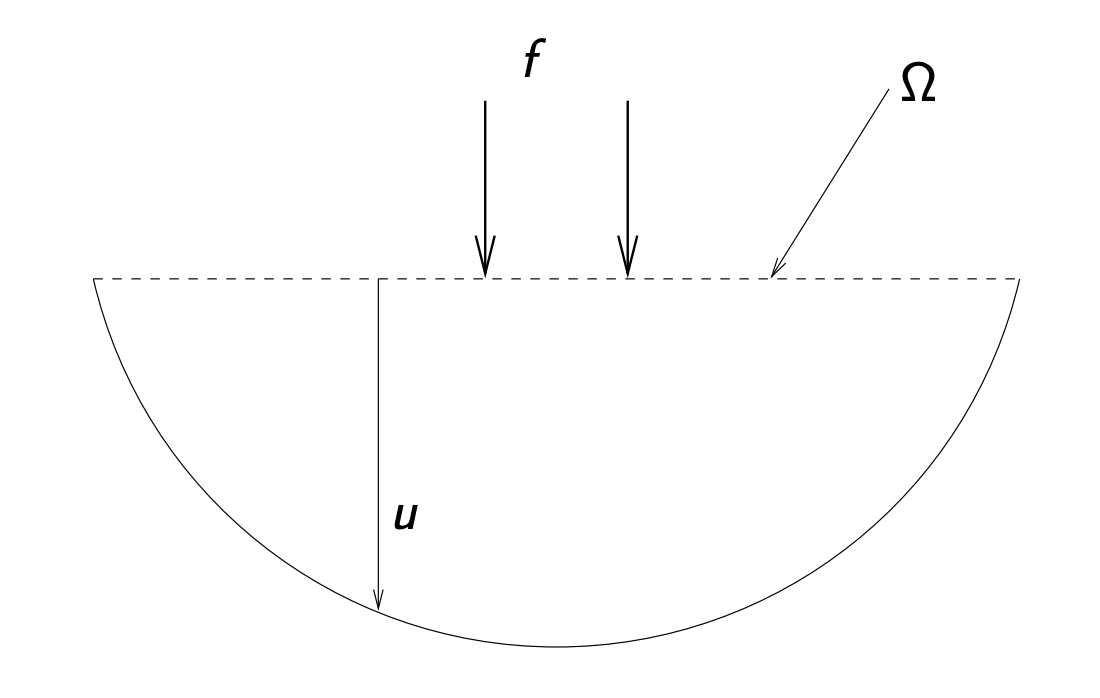
\includegraphics[scale=0.2]{corde00.png} 
\end{center}
\begin{itemize}
\item corde tendue occupant le domaine $\Omega= ]0, 1[$
\item fixée à ses 2 extrémités
\item on applique un chargement vertical $f$
\end{itemize}

\item L'inconnue est le déplacement vertical de la corde $u : \Omega \to \mathbb{R}$
\item Formulation variationnelle
\begin{equation}
\left\{
\begin{array}{l}
\mbox{Trouver } u \in H_0^1(\Omega)\;\mbox{ tel que }\\
\displaystyle \int_{\Omega} u'\cdot  v' = \int_{\Omega}f v \quad \forall v\in H_0^1(\Omega) 
\end{array}
\right.
\label{formVar1}
\end{equation}
\end{itemize}
\end{frame}

%%%%%%%%%%%%%%%%%%%%%%%%%%%%%%%%%%%%%%%%%%%%%%%%%%%%%
\begin{frame}
\frametitle{Construction de l'espace $V_h$}

\begin{description}
\item[Etape 1]: mailler le domaine $\Omega$
\begin{center}
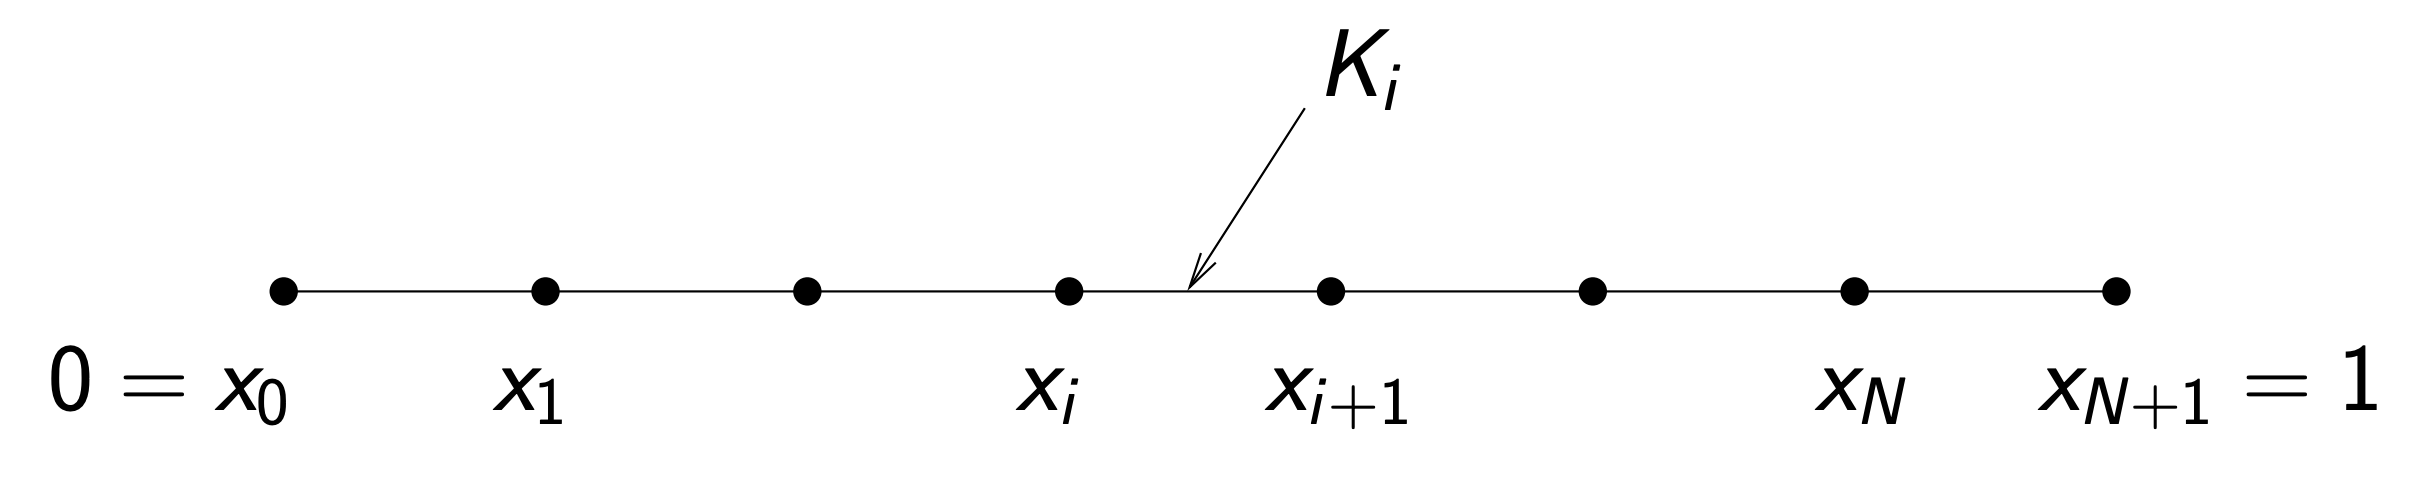
\includegraphics[scale=0.2]{mailleD1.png} 
\end{center}
\begin{itemize}
\item un maillage de $\Omega$ est défini par la donnée de $N$ points distincts dans $\Omega$
\item $(N + 1)$ mailles $K_i = [x_i, x_{i+1}]$,  $\forall i \in\{0\cdots N\}$
\item maillage uniforme : $h = 1/(N + 1)$, $x_i = ih$, $\forall i \in\{0\cdots (N+1)\}$
\end{itemize}
\item[Etape 2]: fixer un comportement (simple) dans chaque maille
\begin{itemize}
\item Fonctions affines par morceaux
\[\{v_h : \Omega \to \mathbb{R}; \; \forall i \in  \{0\cdots N\}, \; v_h|K_i \in \mathbb{P}_1\}\]
où $\mathbb{P}_1= \{p(x) = ax + b;\; a, b \in\mathbb{R}\}$
\item A-t-on la conformité dans $H^1_0(\Omega)$?
\end{itemize}
\end{description}
\end{frame}


%%%%%%%%%%%%%%%%%%%%%%%%%%%%%%%%%%%%%%%%%%%%%%%%%%%%%
\begin{frame}
\frametitle{Construction de l'espace $V_h$}


\begin{itemize}
\item Il faut imposer la nullité au bord
\item Il faut imposer la continuité sur $\Omega$
\[V_h^{(1)}=\{v_h\in C^0(\overline{\Omega});\; \forall i\in\{0\cdots N\},\;v_h\in \mathbb{P}_1;\; v_h(0)=v_h(1)=0\}\]
\item On a $V_h^{(1)}\subset H^1_0(\Omega)$
\item Pour tout $v_h \in V_h^{(1)}$, $v'_h$ est constante par morceaux, obtenue en dérivant maille par maille
\begin{center}
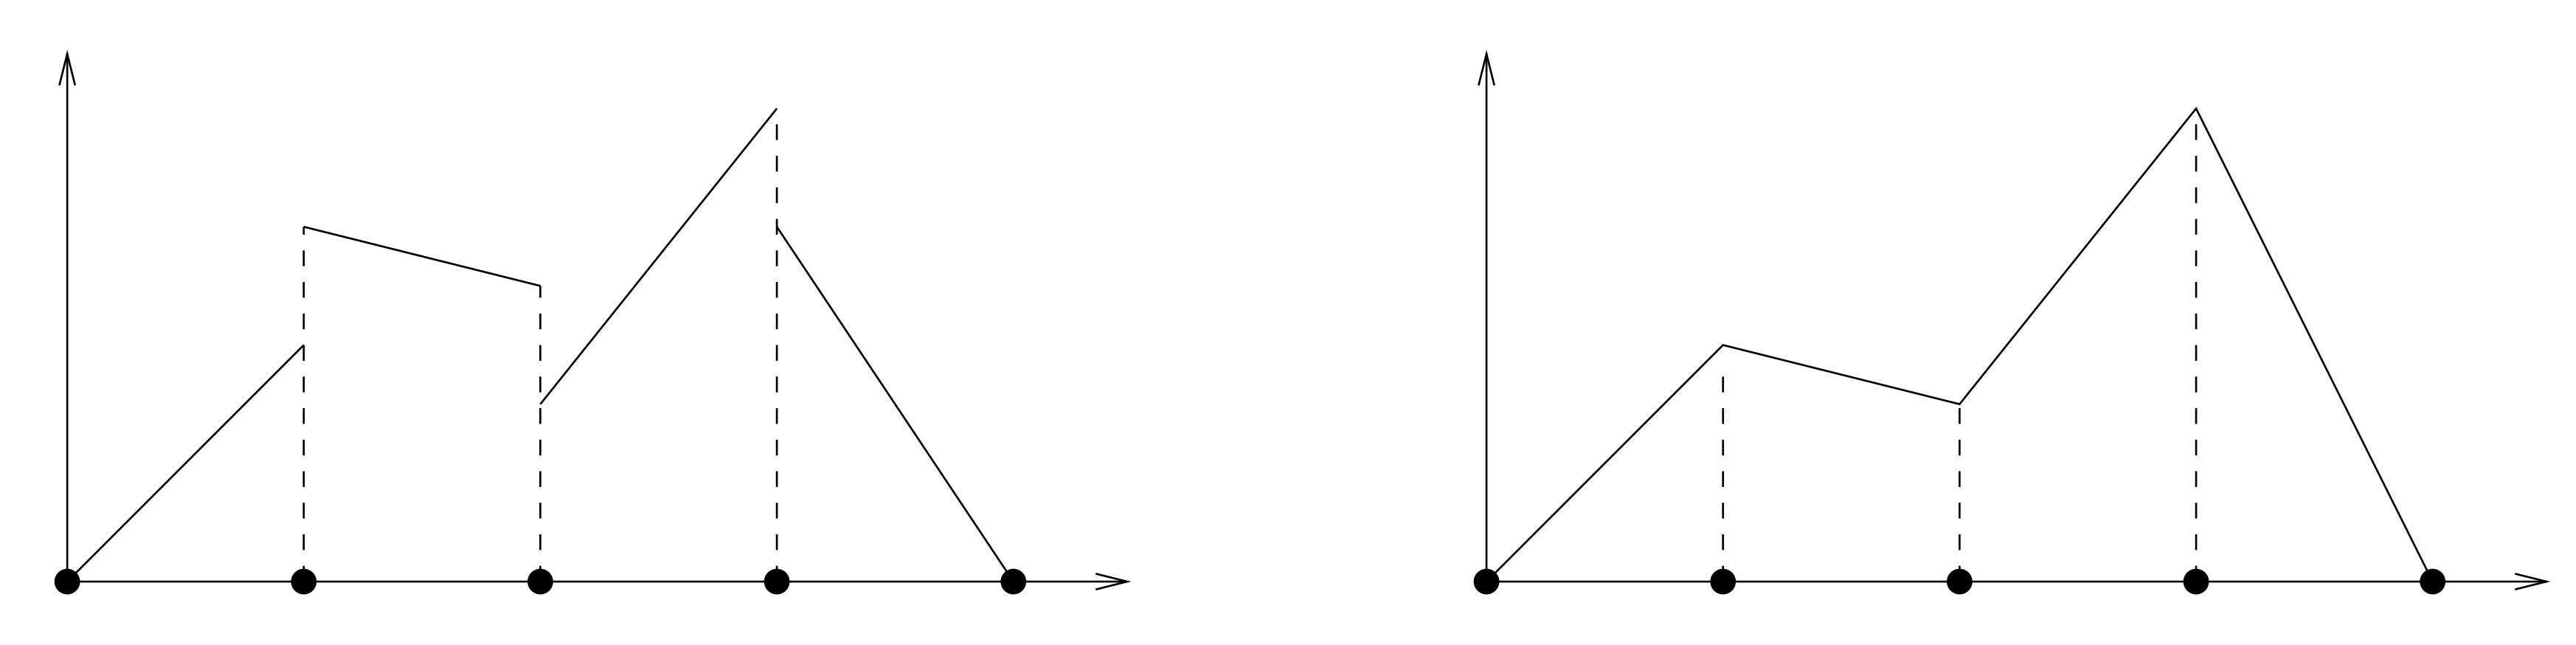
\includegraphics[scale=0.18]{VhD1.png} 
\end{center}
\end{itemize}

\end{frame}

%%%%%%%%%%%%%%%%%%%%%%%%%%%%%%%%%%%%%%%%%%%%%%%%%%%%%
\begin{frame}
\frametitle{Fonctions chapeau}


\begin{itemize}
\item Fonctions chapeau $\{\varphi_1 \cdots \varphi_N \}$
\begin{center}
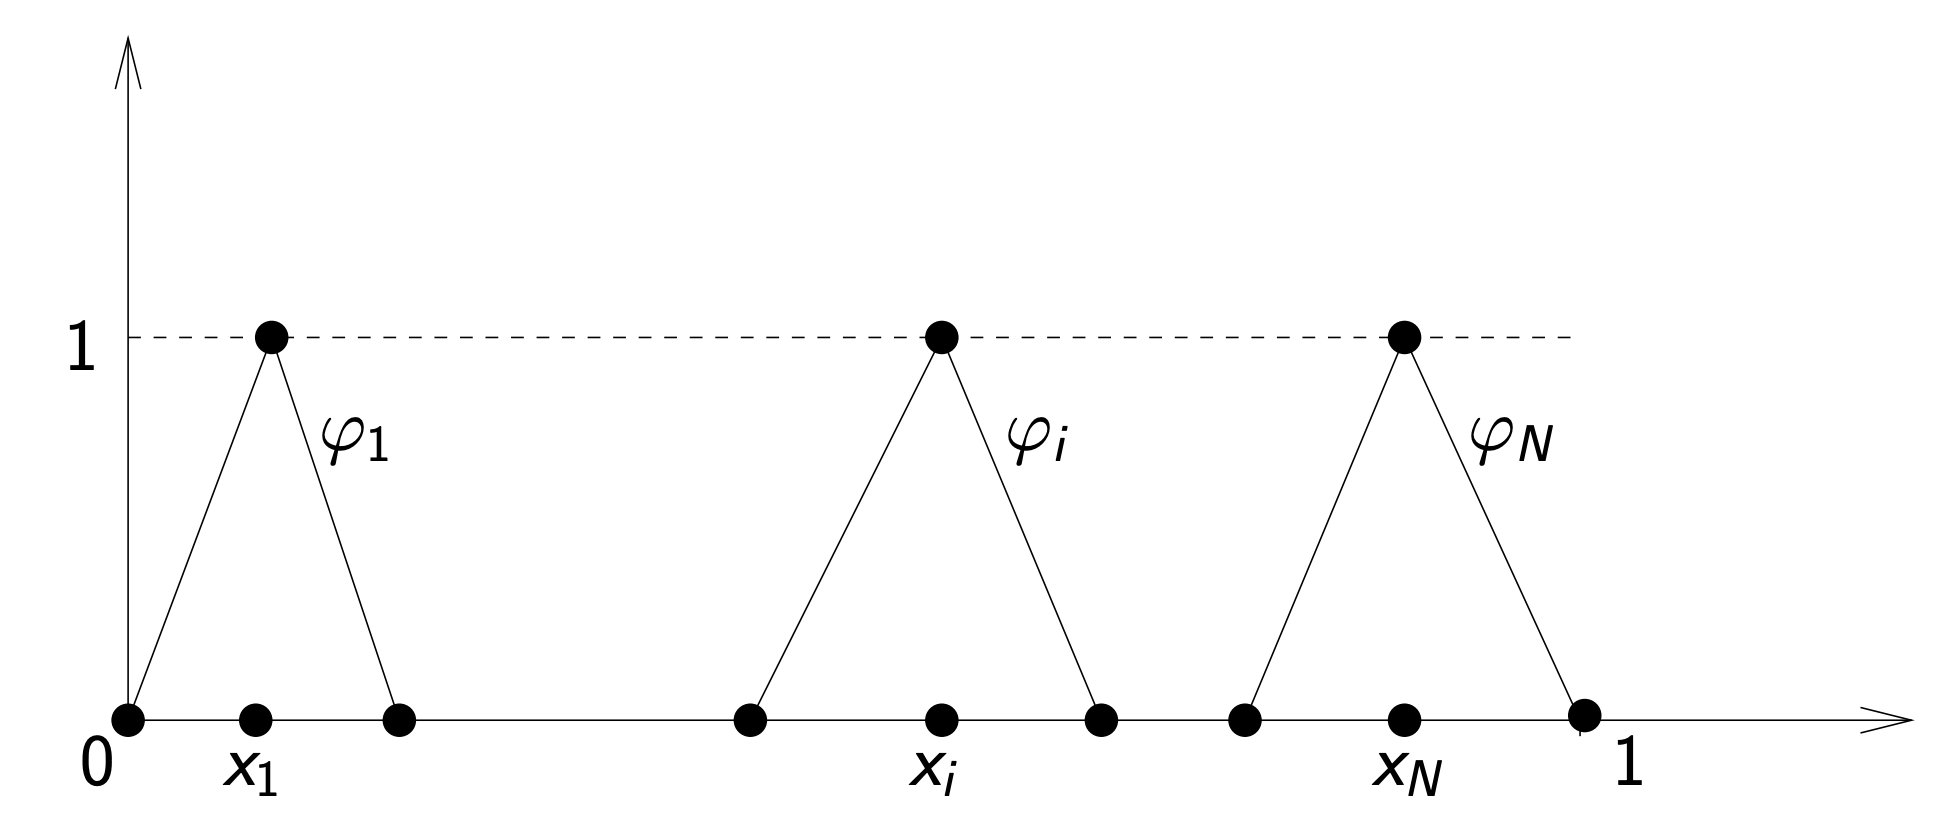
\includegraphics[scale=0.18]{varphiD1.png} 
\end{center}

\item On a $\varphi_i\in V_h^{(1)}$ et $\varphi_i(x_j)=\delta_{ij}$, $\forall i,j\in \{1 \cdots N \}$
\[\varphi_i(x)=\left\{\begin{array}{ll}
\frac{x-x_{i-1}}{h}& x\in K_{i-1}\\
\frac{x_{i+1}-x}{h}& x\in K_{i}\\
0&\mbox{sinon}
\end{array}\right. \quad \varphi'_i(x)=\left\{\begin{array}{ll}
\frac{1}{h}& x\in K_{i-1}\\
-\frac{1}{h}& x\in K_{i}\\
0&\mbox{sinon}
\end{array}\right. \]
\end{itemize}

\end{frame}
%%%%%%%%%%%%%%%%%%%%%%%%%%%%%%%%%%%%%%%%%%%%%%%%%%%%%
\begin{frame}
\frametitle{Base de $V_h$}
\begin{itemize}
\item $\dim(V_h^{(1)})=N$ et $\{\varphi_1 \cdots \varphi_N \}$ est une base de $V_h^{(1)}$

\item La famille est libre : $\forall (\alpha_1 \cdots \alpha_N ) \in \mathbb{R}^N$,
\[\begin{array}{lll}
\displaystyle \sum_{i=1}^N\alpha_i\varphi_i(x)=0&\Longrightarrow & \sum_{i=1}^N\alpha_i\varphi_i(x_j)=0\quad \forall j\in \{1\cdots N\}\\
&\Longrightarrow & \alpha_j=0\quad \forall j\in \{1\cdots N\}
\end{array}\]
\item  La famille est génératrice : $\forall v_h \in V_h^{(1)}$,
\[v_h(x)=\sum_{i=1}^Nv_h(x_i)\varphi_i(x)\]
\begin{itemize}
\item ces deux fonctions sont affines par morceaux
\item elles coïncident en deux points distincts sur chaque maille
\end{itemize}
\end{itemize}

\end{frame}

%%%%%%%%%%%%%%%%%%%%%%%%%%%%%%%%%%%%%%%%%%%%%%%%%%%%%
\begin{frame}
\frametitle{Assemblage de la matrice de rigidité (1)}
\begin{itemize}
\item Rappel du terme générique
\[A_{ij}=a(\varphi_j,\varphi_i)=\int_{\Omega}\varphi'_i(x)\varphi'_j(x)\,\de x\]
\item Observation essentielle : $A_{ij}\neq 0$ seulement si l'intersection des supports de $\varphi_i$ et $\varphi_j$ est de mesure non-nulle
\item La matrice de rigidité est tridiagonale
\[A=\left(\begin{array}{ccccc}
* & * & 0 &\cdots & 0 \\
* & * & *& \ddots & \vdots  \\
0 & \ddots  & \ddots & \ddots & 0 \\
\vdots & \ddots  & * & * & *  \\
0 & \cdots  & 0 & * & * 
\end{array}\right)\]
\item Que valent les coefficients diagonaux et extra-diagonaux?
\end{itemize}


\end{frame}

%%%%%%%%%%%%%%%%%%%%%%%%%%%%%%%%%%%%%%%%%%%%%%%%%%%%%
\begin{frame}
\frametitle{Assemblage de la matrice de rigidité (2)}
\begin{itemize}
\item On calcule le coefficient diagonal
\[\begin{array}{ll}
A_{ii}&=\displaystyle \int_{\Omega}\varphi'_i(x)\varphi'_i(x)\,\de x=\int_{K_{i-1}\cup K_i}(\varphi'_i(x))^2\,\de x\\
&=\displaystyle \int_{K_{i-1}}\cdots+\int_{K_{i}}\cdots=h\times \left(\frac 1h\right)^2+h\times \left(-\frac 1h\right)^2=\frac 2h
\end{array}
\]
\item De même, $A_{i,i-1}=A_{i-1,i}=-\frac 1h$
\item Au final
\[A=\left(\begin{array}{ccccc}
2 & -1 & 0 &\cdots & 0 \\
-1 & 2 & -1& \ddots & \vdots  \\
0 & \ddots  & \ddots & \ddots & 0 \\
\vdots & \ddots  & -1 & 2 & -1  \\
0 & \cdots  & 0 & -1 & 2 
\end{array}\right)\]
\item En 1D, $A$ a les dimensions de l'inverse d'une longueur
\end{itemize}


\end{frame}

%%%%%%%%%%%%%%%%%%%%%%%%%%%%%%%%%%%%%%%%%%%%%%%%%%%%%
\begin{frame}
\frametitle{Interpolation}
\begin{itemize}
\item Opérateur d'interpolation ($H^1_0(\Omega) \subset C^0(\overline{\Omega})$ en 1D)

\[\begin{array}{cccl}
I_h^{(1)}:&H^1_0(\Omega) &\to &V_h\\
& v&\mapsto &\sum_{i=1}^Nv(x_i)\varphi
\end{array}
\]
$I_h^{(1)} v$  prend la même valeur que $v$ en tous les sommets du maillage
\begin{center}
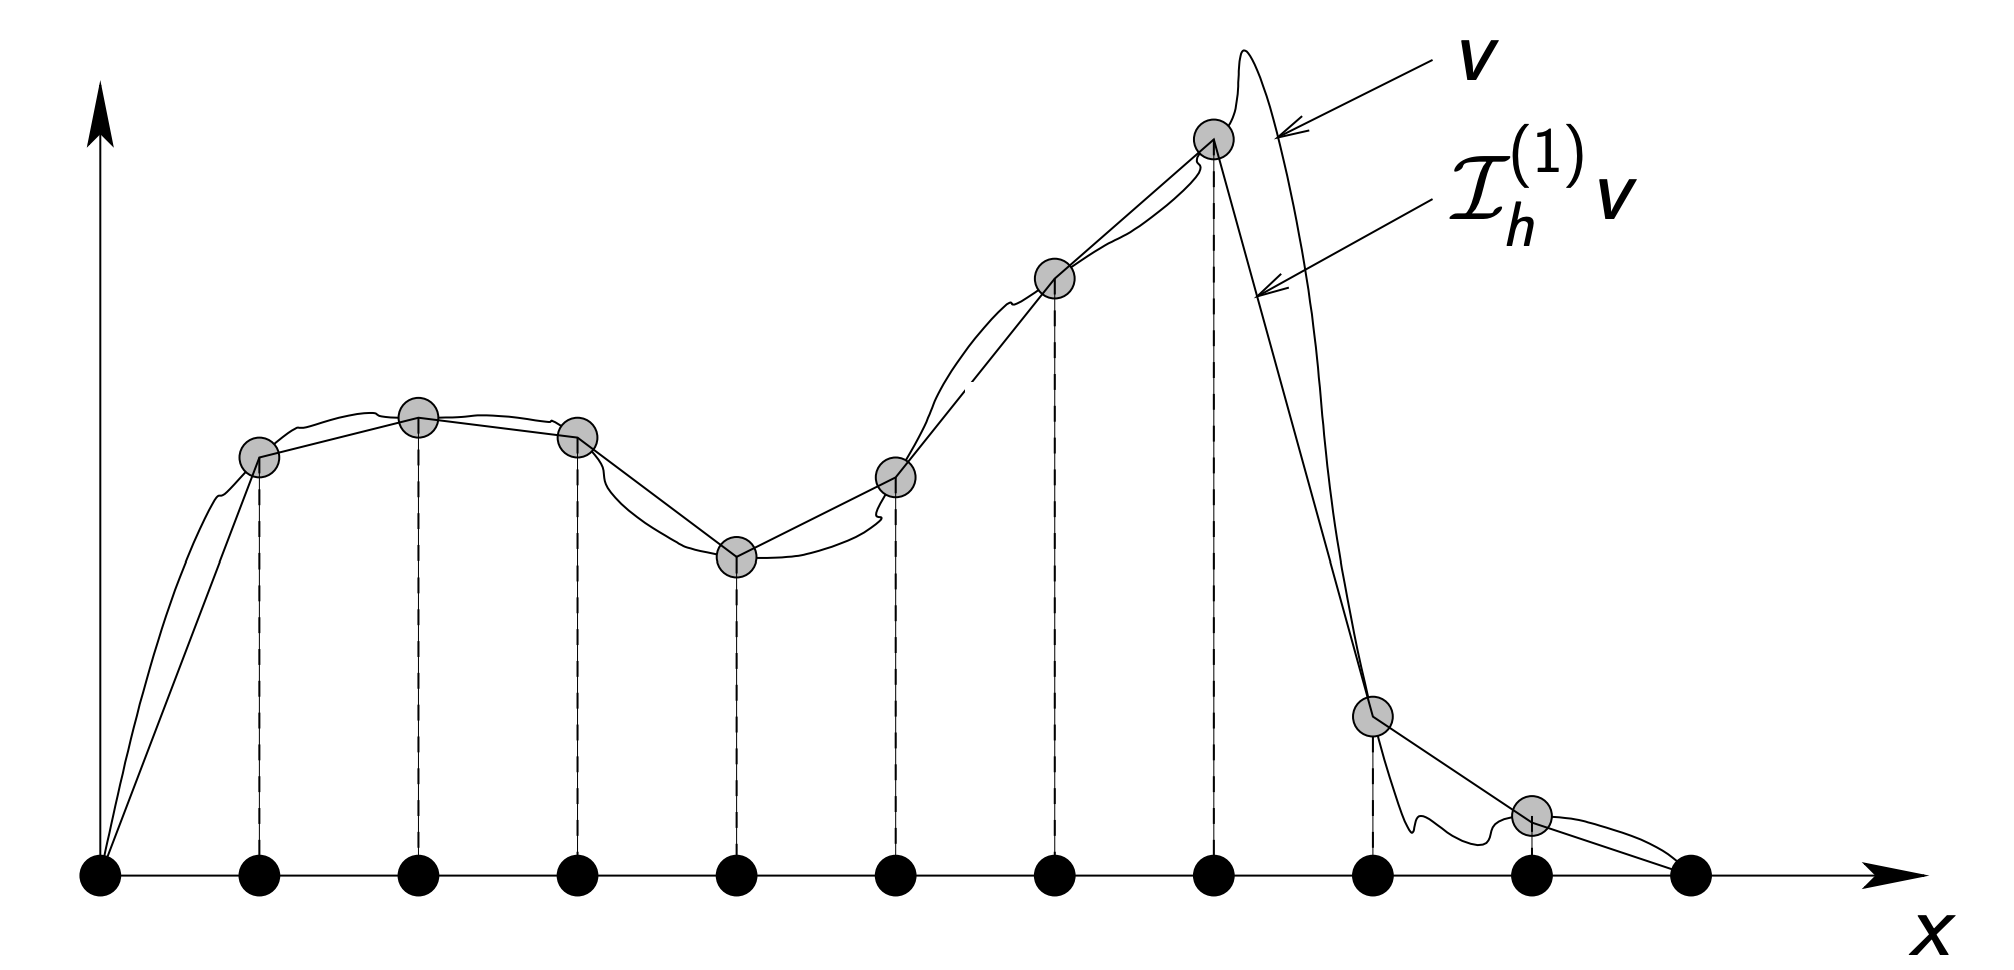
\includegraphics[scale=0.18]{interpolation00.png} 
\end{center}
\item Théorème d'interpolation : $\exists C_{I}$ t.q. $\forall v\in H^2(\Omega) \cap H^1_0(\Omega)$, 

\[\|v'-(I_h^{(1)} v)'\|_{L^2}\leq C_{I} h \|v''\|_{L^2} \]
v s'écarte de son interpolé affine lorsque sa courbure est grande.
\end{itemize}


\end{frame}

%%%%%%%%%%%%%%%%%%%%%%%%%%%%%%%%%%%%%%%%%%%%%%%%%%%%%
\begin{frame}
\frametitle{Applications en dimension n = 2}
\begin{itemize}
\item On considère le problème de Dirichlet

\begin{equation}
\left\{
\begin{array}{l}
-\Delta u= f \mbox{ dans } \Omega,\\
u=0 \mbox{ sur } \Gamma=\partial\Omega,
\end{array}
\right.
\label{dirichletDim2}
\end{equation}
où $\Omega = ]0,1[\, \times \,  ]0,1[$ et  $f\in {\cal C}^0(\overline{\Omega})$.
\item la formulation variationnelle de ce problème consiste à chercher $u\in V=H^1_0(\Omega)$ solution de
\begin{equation}
\forall v_h\in H^1_0(\Omega),\quad a(u,v)=\int_{\Omega} f v\,\de x
\label{dirichletDim2Variationnel}
\end{equation}

où

\begin{equation}
a(u,v)=\int_{\Omega}\left(\frac{\partial u}{\partial x_1}\frac{\partial v}{\partial x_1}+\frac{\partial u}{\partial x_2}\frac{\partial v}{\partial x_2}\right)\de x
\end{equation}
\end{itemize}


\end{frame}

%%%%%%%%%%%%%%%%%%%%%%%%%%%%%%%%%%%%%%%%%%%%%%%%%%%%%
\begin{frame}
\frametitle{Le maillage rectangulaire}
\begin{itemize}
\item les nœuds sont les points $x_{l,m}=(lh,mh)$, $0\leq l,m\leq M+1$;
\item $K_i=\{x_{l,m},x_{l+1,m},x_{l+1,m+1},x_{l,m+1}\}$ est le carré élémentaire de côté $h$.
\item Le maillage est "presque" une partition du domaine $\overline{\Omega}$
\begin{equation}
\left\{
\begin{array}{l}
\displaystyle \overline{\Omega}=\displaystyle \bigcup_{0\leq l,m\leq M}K_{l,m}\\
\mbox{ avec }(l_1,m_1)\neq (l_2,m_2) \Longrightarrow  \mathring{K}_{l_1,m_1}\cap \mathring{K}_{l_2,m_2} = \varnothing\\
\end{array}
\right.
\end{equation}
\begin{center}
\begin{tikzpicture}[domain=0:5,scale=0.90]
 \pgfmathsetmacro{\alpha}{0.05}
  \pgfmathsetmacro{\a}{0.8}
  \draw[->] (0,0) -- (6*\a,0)  node[right] {$x$};
  \draw[->] (0,0) -- (0,5.5*\a) node[left] {$y$};

  \foreach \n in {0,1,...,5}{
   \draw[blue,thick](\n*\a,0)-- ++(0,5*\a);
    \draw[blue,thick](0,\n*\a)-- ++(5*\a,0);
}
\draw (2*\a,0)  node[below] {$\scriptstyle  \ell h$};
\draw (0,3*\a)  node[left] {$\scriptstyle  m h$};

\draw[fill=orange!30] (2*\a,3*\a)  -- ++(\a,0) -- ++(0,\a) -- ++(-\a,0) -- ++(0,-\a);
  \draw (2*\a,3.5*\a)  node[above,right] {$\scriptstyle  K_{l,m}$};
\end{tikzpicture}

\end{center}

\end{itemize}


\end{frame}


%%%%%%%%%%%%%%%%%%%%%%%%%%%%%%%%%%%%%%%%%%%%%%%%%%%%%
\begin{frame}
\frametitle{L'espace des polynômes d'interpolation $Q_1$}
\begin{itemize}
\item $Q_1=\mbox{ vect }(1,x_1,x_2,x_1x_2)$;
\item une fonction $v$ de $Q_1$ est déterminée de manière unique par ses valeurs aux sommets d'un carré $K_{l,m}$.
\item la restriction de $v$ à un côté du carré $K_{l,m}$ est une fonction affine et il suffit donc d'assurer la continuité de $v$ aux extrémités du côté pour que la fonction $v$ soit continue sur tout ce côté. 
\item Donc Ainsi la fonction $v$ est continue sur $\overline{\Omega}$ si et seulement si elle est continue aux  $(M+ 2)^2$ points $a_{l,m}$,  $0\leq l,m\leq M+1$.
\item Par ailleurs, la fonction $v$ est nulle sur $\Gamma$ si et seulement si elle s'annule aux $4(M+ 1)$ points $a_{l,m}$ situés sur $\Gamma$.
\end{itemize}


\end{frame}

%%%%%%%%%%%%%%%%%%%%%%%%%%%%%%%%%%%%%%%%%%%%%%%%%%%%%
\begin{frame}
\frametitle{Approximation: $V_h$}
\begin{itemize}
\item $V\simeq V_h = \{ v\in {\cal C}^0(\overline{\Omega});\; v|_{\Gamma} = 0;\; v|_{K_{l,m}} \in Q_1,\; 0\leq l,m\leq M\}$
\item  Une fonction de l'espace $V_h$ est déterminée de manière unique par les valeurs qu'elle prend en les points $a_{l,m}$ , $1\leq l,m\leq M$.  $\dim V_h=M^2$
\item On numérote de 1 à $M^2$ les points $a_{l,m}$ par la bijection
\begin{equation}
{\cal N}: (l,m)\mapsto i=l+M(m-1)
\end{equation}
\begin{center}
\begin{tikzpicture}[domain=0:5]
 \pgfmathsetmacro{\alpha}{0.05}
  \pgfmathsetmacro{\a}{0.6}
  \pgfmathsetmacro{\M}{4}
  \draw[->] (0,0) -- (6*\a,0)  node[right] {$x$};
  \draw[->] (0,0) -- (0,5.5*\a) node[left] {$y$};


  \foreach \l in {1,...,\M}{
  \foreach \m in {1,...,\M}{
  \pgfmathsetmacro{\i}{int(\l+\M*(\m-1))}
   \draw[blue,thick](\l*\a,\m*\a) node{$\scriptstyle  a_{\i}$};
}
}

\draw[blue,thick] (0,0) -- ++(5*\a,0) -- ++(0,5*\a) -- ++(-5*\a,0) -- ++(0,-5*\a);

\draw (2*\a,0)  node[below] {$\scriptstyle  \ell h$};
\draw (0,3*\a)  node[left] {$\scriptstyle  m h$};

\end{tikzpicture}
\end{center}

 \item On pose $a_i=a_{{\cal N}^{-1}(i)}$
\end{itemize}


\end{frame}

%%%%%%%%%%%%%%%%%%%%%%%%%%%%%%%%%%%%%%%%%%%%%%%%%%%%%
\begin{frame}
\frametitle{Approximation: base de $V_h$}
\begin{itemize}
\item Soit $\varphi_i$, $1\leq i\leq M^2$, la fonction de $V_h$, définie par 
\begin{equation}
\varphi_i(a_j)=\delta_{ij},\quad 1\leq i,j \leq M^2.
\end{equation}
\item   La suite des fonctions $\varphi_i$, $1\leq i\leq M^2$, forme une base de $V_h$ 
\item Les composantes dans cette base d'une fonction $v\in V_h$ sont les nombres $v(a_i)$,  $1\leq i\leq M^2$.

 \item le support de la fonction $\varphi_i$ est le carré de côtés parallèles aux axes, de longueur $2h$ et ayant pour centre le point $a_i$.
 \begin{center}
\begin{tikzpicture}[domain=0:5]
 \pgfmathsetmacro{\alpha}{0.05}
  \pgfmathsetmacro{\a}{0.65}
  \draw[->] (0,0) -- (6*\a,0)  node[right] {$x$};
  \draw[->] (0,0) -- (0,5.5*\a) node[left] {$y$};

  \foreach \n in {0,1,...,5}{
   \draw[blue,thick](\n*\a,0)-- ++(0,5*\a);
    \draw[blue,thick](0,\n*\a)-- ++(5*\a,0);
}
\draw (2*\a,0)  node[below] {$\scriptstyle  \ell h$};
\draw (0,3*\a)  node[left] {$\scriptstyle  m h$};
\draw[fill=orange!30, fill opacity=0.6] (2*\a-\a,3*\a-\a)  -- ++(2*\a,0) -- ++(0,2*\a) -- ++(-2*\a,0) -- ++(0,-2*\a);
  \path[fill=gray] (2*\a,3*\a) circle (0.6mm)node[left,below] {$\scriptstyle  a_i$};
\end{tikzpicture}

\end{center}

\end{itemize}


\end{frame}

%%%%%%%%%%%%%%%%%%%%%%%%%%%%%%%%%%%%%%%%%%%%%%%%%%%%%
\begin{frame}
\frametitle{Approximation: $u_h$}
\begin{itemize}
\item On cherche $u_h=\sum_{j=1}^{M^2} u_i\varphi_j \in V_h$, où $u_j=u_h(a_j),\quad 1\leq j \leq M^2$

\item $(u_j)_j$ est solution du système linéaire

\begin{equation}
\myredbox{\sum_{j=1}^I a(\varphi_j,\varphi_i)u_j=\ell(\varphi_i), \quad 1\leq i\leq M^2}
\end{equation}

\item  La matrice $(a(\varphi_j,\varphi_i))_{1\leq i,j \leq I}$ est symétrique et définie positive ; elle est creuse car $a(\varphi_j,\varphi_i)=0$ sauf si les points $a_i$ et $a_j$ sont sommets d'un même carré $K_{l, m}$.  
 \begin{center}
\begin{tikzpicture}[domain=0:5,scale=0.8]
 \pgfmathsetmacro{\alpha}{0.05}
  \pgfmathsetmacro{\a}{0.65}
  \draw[->] (0,0) -- (6*\a,0)  node[right] {$x$};
  \draw[->] (0,0) -- (0,5.5*\a) node[left] {$y$};

  \foreach \n in {0,1,...,5}{
   \draw[blue,thick](\n*\a,0)-- ++(0,5*\a);
    \draw[blue,thick](0,\n*\a)-- ++(5*\a,0);
}
\draw (2*\a,0)  node[below] {$\scriptstyle  \ell h$};
\draw (0,3*\a)  node[left] {$\scriptstyle  m h$};
\draw[fill=orange!30, fill opacity=0.6] (2*\a-\a,3*\a-\a)  -- ++(2*\a,0) -- ++(0,2*\a) -- ++(-2*\a,0) -- ++(0,-2*\a);
  \path[fill=gray] (2*\a,3*\a) circle (0.6mm)node[left,below] {$\scriptstyle  a_i$};
  \draw[fill=olive!30, fill opacity=0.6] (4*\a-\a,2*\a-\a)  -- ++(2*\a,0) -- ++(0,2*\a) -- ++(-2*\a,0) -- ++(0,-2*\a);
  \path[fill=gray] (4*\a,2*\a) circle (0.6mm)node[left,below] {$\scriptstyle  a_j$};
\end{tikzpicture}

\end{center}

\end{itemize}


\end{frame}

%%%%%%%%%%%%%%%%%%%%%%%%%%%%%%%%%%%%%%%%%%%%%%%%%%%%%
\begin{frame}
\frametitle{Matrice du système}
\begin{itemize}
\item Matrice à bande $a(\varphi_j,\varphi_i)=0$ pour $|i-j|>d_{max}=M+1$
 \begin{center}
\begin{tikzpicture}[domain=0:5,scale=0.7]
 \pgfmathsetmacro{\alpha}{0.05}
  \pgfmathsetmacro{\a}{0.65}

  \draw[-] (-0.5,8) -- (8,8);
  \draw[-] (0,8.5) -- (0,0);

  \foreach \x in {0,2,4,6}{
  \pgfmathsetmacro{\y}{\x}
\draw(\x+0.5,8-0.5-\y)node{$*$};
\draw(\x+1,8-0.5-\y)node{$*$};
\draw(\x+0.5,8-1-\y)node{$*$};
\draw(\x+1,8-1-\y)node{$*$};
\draw(\x+1.5,8-1-\y)node{$*$};

\draw(\x+1,8-1.5-\y)node{$*$};
\draw(\x+1.5,8-1.5-\y)node{$*$};
\draw(\x+2,8-1.5-\y)node{$*$};

\draw(\x+1.5,8-2-\y)node{$*$};
\draw(\x+2,8-2-\y)node{$*$};
}

\foreach \x in {2,4,6}{
  \pgfmathsetmacro{\y}{\x-2}
\draw(\x+0.5,8-0.5-\y)node{$*$};
\draw(\x+1,8-0.5-\y)node{$*$};
\draw(\x+0.5,8-1-\y)node{$*$};
\draw(\x+1,8-1-\y)node{$*$};
\draw(\x+1.5,8-1-\y)node{$*$};

\draw(\x+1,8-1.5-\y)node{$*$};
\draw(\x+1.5,8-1.5-\y)node{$*$};
\draw(\x+2,8-1.5-\y)node{$*$};

\draw(\x+1.5,8-2-\y)node{$*$};
\draw(\x+2,8-2-\y)node{$*$};
}

\foreach \x in {0,2,4}{
\pgfmathsetmacro{\y}{\x+2}
\draw(\x+0.5,8-0.5-\y)node{$*$};
\draw(\x+1,8-0.5-\y)node{$*$};
\draw(\x+0.5,8-1-\y)node{$*$};
\draw(\x+1,8-1-\y)node{$*$};
\draw(\x+1.5,8-1-\y)node{$*$};

\draw(\x+1,8-1.5-\y)node{$*$};
\draw(\x+1.5,8-1.5-\y)node{$*$};
\draw(\x+2,8-1.5-\y)node{$*$};

\draw(\x+1.5,8-2-\y)node{$*$};
\draw(\x+2,8-2-\y)node{$*$};
}
\foreach \x in {1,2,...,16}{
\draw(0.5*\x,8+0.2)node{\tiny\x};
}
\foreach \x in {1,2,...,16}{
\draw(-0.2,8-0.5*\x)node{\tiny\x};
}
\foreach \x in {0,2,4}{
  \draw[dashed] (\x+2.25,0) -- ++(0,7.7);
}
\foreach \x in {0,2,4}{
  \draw[dashed] (0.3,\x+1.75) -- ++(7.7,0);
}
\draw[-,olive] (3,7.5) -- (8,2.5);
\draw[-,olive] (0.5,5) -- (5.5,0);
\draw[-,orange] (0.5,7.5) -- (8,0);
\end{tikzpicture}

\end{center}
\item matrice tridiagonale par blocs, les blocs étant eux-mêmes tridiagonaux. \item méthode de Cholesky ou la méthode de surrelaxation par blocs.
\end{itemize}


\end{frame}

%%%%%%%%%%%%%%%%%%%%%%%%%%%%%%%%%%%%%%%%%%%%%%%%%%%%%
\begin{frame}
\frametitle{Le système linéaire}
\begin{itemize}
\item il est agréable désormais de noter les inconnues $u_{l,m}=u_{{\cal N}(l,m)}$
\item $u_{l,m}$ n'est autre que $u_h(a_{l,m})$


\item  Nous posons, 
\[
f_{l,m}=\frac 1{h^2}\int_{\Omega}f\varphi_{l,m}\,\de x,\quad 1\leq l,m\leq M,
\]
\item les calculs élémentaires montrent que le système s'écrit
\[
\left\{\begin{array}{l}
3u_{l,m}-\frac 13\sum_{\alpha,\beta=-1}^{+1}u_{l+\alpha,m+\beta}=h^2f_{l,m},\quad 1\leq l,m\leq M,\\
u_{l,0}=u_{l,M+1}=0,\quad 0\leq l\leq M+1,\\
u_{0,m}=u_{M+1,m}=0,\quad 0\leq m\leq M+1.
\end{array}\right.
\]
\item schéma à 9 points.
\end{itemize}


\end{frame}

%%%%%%%%%%%%%%%%%%%%%%%%%%%%%%%%%%%%%%%%%%%%%%%%%%%%%
\begin{frame}
\frametitle{Le second membre}
\begin{itemize}
\item sauf cas particulier, on sera incapable de calculer les quantités $f_{l,m}$.
\item formule du point central : si $\psi$ est une fonction continue sur le carré $K_{l,m}$ on a la formule de quadrature qui est exacte pour $\psi\in Q_1$:
\begin{equation}
\int_{K_{l,m}}\psi(x)\,\de x = h^2\varphi\left(lh+\frac h2,mh+\frac h2\right)
\end{equation}
\item  on utilisera la même règle dans chacun des 4 carrés de côté $h$ qui constituent le support de la fonction $\varphi_{l,m}$.
\[
\begin{array}{rl}
\displaystyle f_{l,m}=\frac 14&\displaystyle \left\{f\left(lh-\frac h2,mh-\frac h2\right)+f\left(lh-\frac h2,mh+\frac h2\right)\right.\\
&\displaystyle+\left.f\left(lh+\frac h2,mh-\frac h2\right)+f\left(lh+\frac h2,mh+\frac h2\right)\right\}
\end{array}
\]
\item De même, la formule du trapèze se généralise aisément en la formule : 
\begin{equation}
\int_{K_{l,m}}\psi(x)\,\de x =\frac{ h^2}4\left(\psi(a_{l,m})+\psi(a_{l+1,m})+\psi(a_{l+1,m+1})+\psi(a_{l,m+1})\right)
\end{equation}
qui est encore exacte pour $\psi\in Q_1$. 
\end{itemize}


\end{frame}
%%%%%%%%%%%%%%%%%%%%%%%%%%%%%%%%%%%%%%%%%%%%%%%%%%%%%
\begin{frame}
\frametitle{Décomposition de $\overline{\Omega}$ à  l'aide de triangles}
\begin{itemize}
\item En partageant chaque carré $K_{l,m}$ en deux triangles $K_{l,m,1}$ et $K_{l,m,2}$ suivant la diagonale parallèle  à la première bissectrice, 
\begin{center}
\begin{tikzpicture}[domain=0:5,scale=0.8]
 \pgfmathsetmacro{\alpha}{0.05}
  \pgfmathsetmacro{\a}{1.2}
  \draw[->] (0,0) -- (6*\a,0)  node[right] {$x$};
  \draw[->] (0,0) -- (0,5.2*\a) node[left] {$y$};

  \foreach \n in {0,1,...,5}{
   \draw[blue,thick](\n*\a,0)-- ++(0,5*\a);
    \draw[blue,thick](0,\n*\a)-- ++(5*\a,0);
}
  \foreach \n in {0,1,...,5}{
   \draw[blue,thick](\n*\a,0)-- (5*\a,5*\a-\n*\a);
    \draw[blue,thick](0,\n*\a)-- (5*\a-\n*\a,5*\a);
}
\draw (2*\a,0)  node[below] {$\scriptstyle  \ell h$};
\draw (0,3*\a)  node[left] {$\scriptstyle  m h$};
\draw[fill=orange!30, fill opacity=0.6] (2*\a,3*\a)  -- ++(\a,0) -- ++(0,\a) ;
  \path[fill=gray] (2*\a,3*\a) circle (0.6mm)node[left,below] {$\scriptstyle  a_i$};
  \draw[blue] (2.6*\a,3.2*\a) node{$\scriptstyle  K_{l,m,1}$};
  \draw[fill=olive!30, fill opacity=0.6] (2*\a,3*\a)  -- ++(0,\a) -- ++(\a,0) ;
  \draw[blue] (2.4*\a,3.8*\a) node{$\scriptstyle  K_{l,m,2}$};
\end{tikzpicture}
\end{center}

\end{itemize}


\end{frame}

\end{document}



  On a ainsi 


On désigne par $P_1$ l'espace des polynômes à deux variables de degré inférieur  ou égal à 1 ; par conséquent $P_1$ est l'espace de dimension 3 engendré par les  polynômes 1, x1 et x2. Nous choisissons alors pour espace de dimension finie
\begin{equation}
    V_h = \{ v\in {\cal C}^0(\overline{\Omega});\; v|_{\Gamma} = 0;\; v|_{K_{l,m,p}} \in P_1,\; 0\leq l,m\leq M,\; 1\leq p\leq 2\}
    \end{equation}


Par les mêmes raisonnements que ceux qui ont suivi le choix (3.3-8) d'espace $V_h$, on démontre maintenant que l'espace $V_h$ défini par (3.3-25) est un sous-espace de $V=H^1_0(\Omega)$ de dimension finie $I= M^2$, que les nombres $u_{l,m}=u_h(a_{l,m})$, $1\leq l,m\leq M$ déterminent de manière unique une fonction $u_h$ de $V_h$, enfin que la méthode d'approximation variationnelle conduit à résoudre ici le système 

\begin{equation}
-u_{l-1,m}-u_{l,m-1}+4u_{l,m}-u_{l,m+1}-u_{l+1,m}=h^2 f_{l,m},\quad 1\leq l,m\leq M
\end{equation}

avec
\begin{equation}
\left\{\begin{array}{l}
u_{l,0}=u_{l,M+1}=0,\quad 0\leq l\leq M+1,\\
u_{0,m}=u_{M+1,m}=0,\quad 0\leq m\leq M+1.
\end{array}\right.
\end{equation}

où la définition des quantités $f_{l,m}$ est analogue à (3.3-17). Lorsque les intégrales sur chaque triangle $K_{l,m,p}$ sont évaluées à l'aide de la formule de quadrature

 \[
 \int_{K_{l,m,1}}\psi(x)\de x = \frac{h^2}{6}\left[\psi(a_{l,m})+\psi(a_{l+1,m})+\psi(a_{l+1,m+1})\right]
 \]
 \[
 \int_{K_{l,m,2}}\psi(x)\de x = \frac{h^2}{6}\left[\psi(a_{l,m})+\psi(a_{l,m+1})+\psi(a_{l+1,m+1})\right]
 \]
 
les quantités $f_{l,m}$  sont approchées par les valeurs $f(a_{l,m})$.


\chapter{Les éléments finis}
 Au premier paragraphe de ce chapitre, nous introduisons la notion générale d'élément fini de Lagrange. Les deux paragraphes suivants sont consacrés à une description détaillée d'exemples simples, donc fondamentaux, où le domaine géométrique de l'élément fini est soit un n-simplexe (paragraphe 2) soit un $n$-parallélotope (paragraphe 3). L'analyse de l'erreur d'interpolation dans un élément fini est faite au paragraphe 4 ; cette partie étant assez technique, le lecteur pourra (en première lecture) n'en retenir que les corollaires 4.4-1 et 4.4-2.
\section{Éléments finis de Lagrange}
  On se donne :
  \begin{enumerate}
  \item une partie compacte $K$ de $\mathbb{R}^n$, connexe et d'intérieur non vide ; 
  \item un ensemble fini $\Sigma =\{a_j\}_{j=1}^N$ de $N$ points distincts de $K$ ;
  \item un espace vectoriel $P$ de dimension finie et composé de fonctions définies 
sur $K$ à valeurs réelles.
  \end{enumerate}
\begin{definition}
On dit que l'ensemble $\Sigma$ est $P$-unisolvant si et seulement si, étant donné $N$ scalaires réels quelconques $\alpha_j$, $1\leq j \leq N$, il existe une fonction $p$ de l'espace $P$ et une seule telle que
                          \begin{equation}
                          p(a_j)=\alpha_j,\qquad 1\leq j \leq N
                          \end{equation}
\end{definition}    
\begin{definition}
Lorsque l'ensemble $\Sigma$ est $P$-unisolvant, le triplet $(K, P, \Sigma)$ est appelé élément fini de Lagrange.
\end{definition}    
  Étant donné un élément fini $(K, P, \Sigma)$, il existe donc pour tout entier $i$, $1\leq j \leq N$, une fonction $p_i\in P$ et une seule telle que
 \begin{equation}
                          p_i(a_j)=\delta_{ij},\qquad 1\leq j \leq N
                          \label{unisolvantCarac}
\end{equation}

Plus généralement pour toute fonction $v$ définie sur $K$ à valeurs réelles, il existe une fonction $p\in P$ et une seule qui interpole $v$ sur $\Sigma$, c'est-à-dire qui satisfait
 \begin{equation}
                          p(a_j)=v(a_j),\qquad 1\leq j \leq N
                          \label{conditionNoeud}
\end{equation}
\begin{definition}
Étant donné un élément fini de Lagrange $(K, P, \Sigma)$, on appelle fonctions de base les $N$ fonctions $p_i$, $1\leq j \leq N$, définies par (4.1-2). On appelle opérateur de $P$-interpolation de Lagrange sur $\Sigma$ l'opérateur qui à toute fonction $v$ définie sur $K$ associe la fonction $\Pi v$ définie par
\begin{equation}
\Pi v = \sum_{i=1}^Nv(a_i)\,p_i,
\label{interpolation}
\end{equation}
et $\Pi v$ est dit le $P$-interpolé de Lagrange de $v$ sur $\Sigma$. 
\end{definition}  

En effet la fonction $\Pi v$ définie par \eqref{interpolation} vérifie
\[(\Pi v)(a_j)=\sum_{i=1}^Nv(a_i)\,\delta_{ij}=v(a_j),\qquad 1\leq j \leq N \]
c'est donc l'unique fonction $p$ de $P$ vérifiant \eqref{conditionNoeud}.

Une condition nécessaire évidente pour que l'ensemble X soit 
P-unisolvant est que
\begin{equation}
\dim(P)=\mbox{card}(\Sigma)=N
\label{condNecessaire}
\end{equation}

Dès que cette condition nécessaire \eqref{condNecessaire} est vérifiée, nous avons deux critères 
simples de $P$-unisolvance pour $\Sigma$ :
\begin{enumerate}
\item  Il suffit de vérifier que la seule fonction de $P$ qui s'annule sur $\Sigma$ est la fonction identiquement nulle. En effet, lorsque cette propriété est satisfaite, l'application linéaire 2 définie de $P$ dans $\mathbb{R}^N$ par
\begin{equation}
{\cal L}(p)=(p(a_j))_{j=1}^N
\end{equation}
est injective, donc bijective puisque $P$ est de dimension $N$.
\item   Il suffit encore d'exhiber les fonctions $p_i$, $1\leq i \leq N$, de l'espace $P$ qui vérifient \eqref{unisolvantCarac} (ce seront alors les fonctions de base) pour prouver la $P$-unisolvance de $\Sigma$. 

En effet, si ces fonctions $p_i$ existent, à toute donnée de $N$ scalaires réels $a_i$, $1\leq i \leq N$, on associe la fonction 
\[p=\sum_{j=1}^N\alpha_jp_j\]
Cette fonction est une fonction de $P$ telle que
 \[p(a_j)=\alpha_j,\quad 1\leq i \leq N \]
Ceci prouve que l'application linéaire ${\cal L}$ considérée précédemment est surjective donc bijective.
\end{enumerate}

         La connaissance des fonctions de base sera fondamentale ; aussi utiliserons-nous dans les exemples donnés ci-après le deuxième critère. Néanmoins il est vivement recommandé de ne pas négliger le premier critère : il a l'avantage d'être souvent de vérification beaucoup plus rapide et justifie alors a priori que les efforts entrepris pour calculer les fonctions de base ne sont pas faits en vain.
         
         Donnons maintenant une méthode systématique pour générer à partir d'un 
élément fini $(K, P, \Sigma)$ toute une famille d'éléments finis. Soit $\widehat{K}$ une partie compacte de $\mathbb{R}^n$, connexe, d'intérieur non vide et soit $F$ une application de $\widehat{K}$ dans $\mathbb{R}^n$. On suppose que
\begin{equation}
K=F(\widehat{K})
\end{equation}
est une partie compacte, connexe et d'intérieur non vide (dès que $F$ est une bijection bicontinue de $\widehat{K}$ sur $K$, ces hypothèses sur $K$ résultent de celles faites sur $\widehat{K}$).

 \begin{theorem}
On suppose l'application $F$ injective. Alors si $(\widehat{K}, \widehat{P}, \widehat{\Sigma})$ est un élément fini de Lagrange, le triplet $(K, P, \Sigma)$, où $K$ est défini par (4.1-5) et où 
on a posé
\begin{equation}
P=\{p:K\to\mathbb{R};\; p\circ F\,\in \widehat{P}\},
\end{equation}
\begin{equation}
\Sigma = F(\widehat{\Sigma})),
\end{equation}
est un élément fini de Lagrange.
\end{theorem}         

\begin{definition}
Deux éléments finis de Lagrange $(\widehat{K},\widehat{P},\widehat{\Sigma})$ et $(K, P, \Sigma)$ sont dits équivalents s'il existe une bijection $F$ de $\widehat{K}$ sur $K$ vérifiant (4.1-6) et (4.1-7) ; de plus, lorsqu'on peut choisir pour une telle bijection $F$ une application affine 
inversible, les éléments finis sont dits affine-équivalents.
\end{definition}  
\begin{theorem}
Soit$(\widehat{K},\widehat{P},\widehat{\Sigma})$ et $(K, P, \Sigma)$ deux éléments finis de Lagrange équivalents et $F$ une bijection de $\widehat{K}$ sur $K$  vérifiant (4.1-6) et (4.1-7). Si $\widehat{\Pi}$ est l'opérateur de :$\widehat{P}$-interpolation sur $\widehat{\Sigma}$, l'opérateur $\Pi$ de $P$-interpolation sur $\Sigma$ est caractérisé par
\begin{equation}
(\Pi v)\circ F = \widehat{\Pi}(v\circ F)
\end{equation}
pour toute fonction $v$ définie sur $K$, c'est-à-dire
\begin{equation}
\widehat{\Pi v} =\widehat{\Pi} \widehat{v}
\end{equation}
\end{theorem}

\section{Éléments finis simpliciaux}
Nous allons construire une classe d'éléments finis de Lagrange $(K, P,\Sigma)$,                                                                                                      où le domaine géométrique $K$ sera un $n$-simplexe quelconque de $\mathbb{R}$. Auparavant, rappelons la définition d'un $n$-simplexe : On considère $n +1$ points $a_j=(a_{ij})_{i=1}^n\in \mathbb{R}^n$, $1\leq j \leq n+1$, non situés dans un même hyperplan de $\mathbb{R}^n$, c'est-à-dire tels que la matrice d'ordre n +1

\begin{equation}
A=\left(\begin{array}{llll}
a_{11} & a_{12} & \cdots & a_{1,n+1} \\ 
a_{21} & a_{22} & \cdots & a_{2,n+1} \\ 
\vdots& \vdots &  & \vdots \\ 
a_{n1} & a_{n2} & \cdots & a_{n,n+1} \\ 
1 & 1 & \cdots & 1
\end{array}\right)
\end{equation}
soit inversible. On appelle $n$-simplexe $K$ de sommets $a_j$, $1\leq j\leq n+1$,                                                                                                         l'enveloppe convexe des points $a_j$ ; pour $n=2$ (resp. $n = 3$), on reprendra pour $K$ la dénomination usuelle de triangle (resp. tétraèdre).

  Tout point $x$ de $\mathbb{R}^n$, de coordonnées cartésiennes $x_i$, $1\leq i\leq n$, est caractérisé par la donnée des $n+ 1$ scalaires ,$\lambda_j=\lambda_j(x)$, $1\leq j \leq n+1$, définis comme solution du système linéaire

\begin{equation}
\left\{\begin{array}{l}
\displaystyle \sum_{j=1}^{n+1}a_{ij}\lambda_j =x_i, \quad 1\leq i\leq n\\
\displaystyle \sum_{j=1}^{n+1}\lambda_j =1
\end{array}\right.
\label{systLinBarycentrique}
\end{equation}
dont la matrice est précisément la matrice inversible $A$. Ces scalaires $\lambda_j(x)$ sont  appelés les coordonnées barycentriques du point $x$ par rapport aux $n+ 1$ points 
$a_j$, $1\leq j\leq n+1$, Les fonctions
\begin{equation}
x=(x_i)_{1\leq i\leq n}\mapsto \lambda_j(x),\quad 1\leq j \leq n+1,
\end{equation}
sont les fonctions coordonnées barycentriques par rapport aux points $a_j$. D'après \eqref{systLinBarycentrique}, chacune de ces fonctions coordonnées barycentriques est une fonction affine de$\mathbb{R}^n$ dans $\mathbb{R}$ et on a
\begin{equation}
\forall x\in\mathbb{R}^n,\quad x=\sum_{j=1}^{n+1}\lambda_j(x) a_{j}
\end{equation}

A l'aide de ces coordonnées barycentriques par rapport aux points $a_j$, le $n$-simplexe $K$ de sommets $a_j$, $1\leq j\leq n+1$, est caractérisé par
\begin{equation}
K=\{x\in \mathbb{R}^n;\;0\leq \lambda_j(x) \leq 1,\; 1\leq j\leq n+1\}
\end{equation}
  D'autre part, pour tout entier   $k\geq 0$,  on désigne par $P_k$ l'espace des (fonctions) polynômes de $\mathbb{R}^n$ dans $\mathbb{R}$ de degré inférieur ou égal à $k$, c'est-à-dire de la forme
\begin{equation}
\forall x\in\mathbb{R}^n,\quad p(x)=\sum_{\begin{array}{c} i_1\geq 0,\cdots ,i_n\geq 0\\i_1+\cdots +i_n\leq k \end{array}}\alpha_{i_1,\cdots,i_n}x_1^{i_1}\cdots x_n^{i_n},
\end{equation}
où les $\alpha_{i_1,\cdots,i_n}$  sont des scalaires réels.

  L'espace des polynômes à $n$ variables homogènes de degré $k$ est de dimension 
$\binom {n+k-1}k$, nombre de combinaisons avec répétitions de longueur $k$ formées à partir des éléments d'un ensemble de cardinal $n$. Par conséquent, la dimension de l'espace $P_k$ est
\begin{equation}
\dim(P_k)=\sum_{l=0}^k \binom {n+l-1}l=\binom {n+k}k=\frac{(n+k)!}{n!k!}
\end{equation}
  On définit enfin, pour tout entier $k$ le treillis principal d'ordre $k$ du $n$-simplexe $K$ comme étant l'ensemble de points de $\mathbb{R}^n$ défini à l'aide des coordonnées barycentriques par rapport aux sommets $a_j$ par
\begin{equation}
\Sigma_k=\left\{x\in\mathbb{R}^n;\;\lambda_j(x)\in\{0,\frac 1k,\cdots,\frac{k-1}{k},1\}, \;1\leq j\leq n+1\right\}
\end{equation}
  Pour k=0, on posera
\begin{equation}
\Sigma_0=\left\{x\in\mathbb{R}^n;\;\lambda_j(x)=\frac{1}{n+1}, \;1\leq j\leq n+1\right\}
\end{equation}

autrement dit $\Sigma_0$ est réduit à un point, le barycentre de $K$. Plus généralement,  en tenant compte de la relation
\begin{equation}
\lambda_{n+1}=1-\sum_{j=1}^n\lambda_j,
\end{equation}
on vérifie que le cardinal de l'ensemble $\Sigma_k$ est le nombre de combinaisons avec   répétitions de longueur $k$ formées à partir des éléments de $\{0,\cdots,n\}$                                                                                                                                         d'où 
\begin{equation}
\mbox{card}(\Sigma_k)=\binom {(n+1)+k-1}k=\binom {n+k}k=\frac{(n+k)!}{n!k!}
\end{equation}
 \begin{theorem}
 Pour tout entier $k\geq 0$, l'ensemble $\Sigma_k$ , est $P_k$-unisolvant.
 \end{theorem}
\begin{definition}
Pour tout $n$-simplexe $K$ de $\mathbb{R}^n$ et pour tout entier   $k\geq 0$,    l'élément

fini $(K, P_k, \Sigma_k)$, où $\Sigma_k$ est le treillis principal d'ordre $k$ de $K$, est appelé $n$-simplexe de type ($k$).
\end{definition}

\begin{theorem}
Pour tout entier $k\geq 0$, deux éléments finis $n$-simplexes de type ($k$) sont affine-équivalents.
\end{theorem}

D'après ce qui précède, il est clair que tout élément fini de Lagrange $(K, P, \Sigma)$ affine-équivalent à un n-simplexe de type ($k$) est un n-simplexe de type ($k$). Il suffira donc d'étudier les propriétés d'un $n$-simplexe de type ($k$) particulier $(\widehat{K} , \widehat{P} , \widehat{\Sigma})$  appelé $n$-simplexe de référence. Habituellement, tant en théorie qu'en pratique, on choisit pour $\widehat{K}$ le n-simplexe unité de sommets 
$\hat{a}_1= (1 , 0, \cdots, 0)$ , $\hat{a}_2= (0,1 , 0, \cdots, 0)$, ... $\hat{a}_n= (0 , \cdots, 0,1)$, $\hat{a}_{n+1}= (0 , 0, \cdots, 0)$. Dans ce cas, les coordonnées barycentriques sont
\begin{equation}
\hat{\lambda}_i(\hat{x})=\hat{x}_i,\; 1\leq i\leq n;\quad \hat{\lambda}_{n+1}=1-\sum_{i=1}^n\hat{\lambda}_i,
\end{equation}
       Considérons un peu plus en détail les éléments finis $(K, P, \Sigma)$ $n$-simplexes de 
type ($k$) les plus couramment utilisés en pratique.
\begin{enumerate}
\item Lorsque $n=2$, $K$ est le triangle de sommets $a_1$, $a_2$ et $a_3$. On pose
\end{enumerate}
\[\begin{array}{lcl}
a_0&=&\frac{1}{3}(a_1+a_2+a_3)\\
a_{ij}&=&\frac{1}{2}(a_i+a_j),\quad 1\leq i<j\leq 3,\\
a_{iij}&=&\frac{1}{3}(2a_i+a_j),\quad 1\leq i<j\leq 3,\; i\neq j
\end{array}
\]

\end{document}





















